\section{Method}

The following section focuses on the approach taken to fulfill the aims of this project. Firstly, it will look at the requirements derived from the background research and will formulate those into some system requirements. Section 3.2 will look at the design of the program for colouring the graphs and some of the methods used to represent graphs and the algorithms in code. 
Section 3.3 will look closer at the implementation of the program as a whole. Finally, section 3.4 looks at methods of testing and the approach behind the results that were gathered. 
\\\\
As mentioned in previous sections the aim of this project is to create a program for colouring graph instances in DIMACS format, similar to that created by Lewis accompanying his guide to graph colouring \cite{LewisR.M.R2015AGtG}. However, this project will purely focus on constructive colouring algorithms and will include the ability to test on multiple DIMACS instance graphs along with randomly generated graph instances. Lewis' program used C++ as the choice of language to build up the application, however the choice for this project was Java. The choice of language is mainly arbitrary and dependant upon the preference of the developer. However, in this case Java provided particular advantages for this project. The first being that it is the most comfortable language for the author and developer, therefore making it a clear choice. The second reason for choosing Java is to take advantage of the Object-Oriented Programming (OOP) techniques (such as inheritance and abstraction) it provides in creating hierarchies to aid in representation of Graphs, Vertices and Edges. Java also has many inbuilt data-structures within the language that make the implementation of the algorithms quicker and simpler to understand. Overall, the choice mainly came down to the preference of the developer, although the choice of Java also provided some extra benefits in this case. 
\\\\
The development of this project will be completed using agile methodology. Due to the nature of the software being produced there may need to be modifications to the requirements and design during the development phase \cite{Agile}. Also, there is a limited time to complete this project therefore lengthier methodologies, such as waterfall, that involve strict phases of requirements gathering, design, implementation and testing did not seem appropriate in this case \cite{Waterfall}. Using agile will allow for tweaks within the design and requirements while simultaneously implementing and testing the software. Therefore, agile seemed the most appropriate methodology to adopt for this project. 

\subsection{Requirements}
System requirements are an important aspect of the software development process to determine the functionality of the system to be produced. Based on the background research in section 2, and considering the overall aim of the project, the following requirements should be considered in the design of the program as a whole:
\begin{itemize}
    \item Ability to read in graphs from input files in DIMACS format
    \item Ability to store the read in graphs in Adjacency List and Adjacency Matrix format
    \item Ability to colour these graphs using the constructive colouring techniques previously established
    \item Ability to gather results regarding number of colours used, number of operations, and time taken for each algorithm
    \item Ability to print these results to an output file
    \item Ability to generate random $G(n, p)$ graphs
    \item To have a simple User Interface (UI)
\end{itemize}

To include all of these requirements, and given the time constraints of the project, the program to be created will use a simple terminal UI. This will be the way a user can interact with the algorithms and will be used for the generation of the results in section 4 of this project.  

\subsubsection{Functional Requirements}
The functional requirements of the system represent the specific features expected of the system that will allow a user to accomplish the desired tasks. The features required of the UI are listed in the table below.

\begin{longtable}{|m{0.1\textwidth}|m{0.65\textwidth}|m{0.1\textwidth}|m{0.15\textwidth}|}
    \hline
    \textbf{Number} &  \textbf{Description} & \textbf{Priority} & \textbf{Comments} \\
    \hline
    FR1 & User can colour a single graph & High & See NFR1-2 \\
    \hline
     FR2 & User can colour a graph of their choice in DIMACS format using \textbf{GREEDY} algorithm & High & See NFR2 \\
     \hline
     FR3 & User can colour a graph of their choice in DIMACS format using \textbf{SHUFFLED GREEDY} algorithm & High & See NFR2 \\
     \hline
     FR4 & User can colour a graph of their choice in DIMACS format using \textbf{WELSH-POWELL1} algorithm & High & See NFR2 \\
     \hline
     FR5 & User can colour a graph of their choice in DIMACS format using \textbf{WElSH-POWELL2} algorithm & High & See NFR2 \\
     \hline
     FR6 & User can colour a graph of their choice in DIMACS format using \textbf{DSATUR} algorithm & High & See NFR2 \\
     \hline
     FR7 & User can colour a graph of their choice in DIMACS format using \textbf{RLF} algorithm & High & See NFR2 \\
     \hline
     FR8 & User can colour a graph of their choice in DIMACS format using all of the algorithms & High & See NFR2 \\
     \hline
     FR9 & User can generate results from testing all algorithms on DIMACS challenge instance graphs & High & See NFR3\\
     \hline
     FR10 & User can generate results from testing all algorithms on randomly generated $G(n, p)$ graphs & High & See NFR4\\
     \hline
     FR11 & User can generate a new random $G(n, p)$ graph & Medium & See NFR5 \\
    \hline
    FR12 & Users can choose to use algorithms with either adjacency list graphs or adjacency matrix graphs as input & Medium & \\
     \hline
     FR13 & User can exit the program & High & See NFR6\\
     \hline
\caption{Functional Requirements}
\label{tab:FuncReqs}  
\end{longtable}
  

\subsubsection{Non-Functional Requirements}
The non-functional requirements specify and describe the systems capabilities and constraints. These are listed in the table below. 

\begin{longtable}{|m{0.1\textwidth}|m{0.65\textwidth}|m{0.1\textwidth}|m{0.15\textwidth}|}
\hline
\textbf{Number} &  \textbf{Description} & \textbf{Priority} & \textbf{Comments} \\
\hline
NFR1 & The users will be provided with a menu to choose if they would like to: 
        \begin{enumerate}
            \item colour a single graph
            \item generate results from a set of DIMACS challenge instances
            \item generate results from a set random $G(n, p)$ instances
            \item generate a random $G(n, p)$ instance
            \item exit the program
        \end{enumerate}
        Any invalid input will ask for a reentry.
        & High & Satisfies FR1,9,10,11,12  \\
\hline
NFR2 & Users can colour a single graph using any of the implemented algorithms by:
        \begin{enumerate}
            \item selecting option 1 in the main menu
            \item inputting the file path of the graph to colour
            \item selecting which (or all) algorithm to use  
        \end{enumerate}
        If the graph is not in DIMACS format or cannot be found users will be asked to start again.
        Results will be printed to the terminal. Time taken to produce results will depend on size and density of input graph.
        & High & Satisfies FR1-8 \\
\hline
NFR3 & Results can be generated for DIMACS instances by selecting option 2 in the main menu. The user will then need to input the number of test runs required for each graph. The results will be printed to an output file and the name of the file printed to the terminal. Results will be gathered regarding number of colours used, number of operations and time taken. The time taken to complete generating results depends on the number of test runs desired. & High & Satisfies FR9 \\
\hline
NFR4 & Results can be generated for $G(n, p)$ graphs by:
    \begin{enumerate}
        \item selecting option 3 in the main menu
        \item input number of $G(n, p)$ graphs to generate per $p$-value
        \item input comma separated list of $p$-values
        \item input number of $n$
    \end{enumerate}
    Any invalid input the user will need to restart. Results will be printed to an output file and the name of the file will be printed to the terminal. Results will be gathered regarding number of colours used, number of operations and time taken. Time taken to complete generating results depends on number of graphs generated, number of $p$-values being tested and size of $n$.
    & High & Satisfies FR10 \\
\hline
NFR5 & A random $G(n, p)$ can be generated by:
    \begin{enumerate}
        \item selecting option 4 from the main menu
        \item input a value for $n$
        \item input a value for $p$
    \end{enumerate}
    Any invalid input the user will need to restart. The graph will be printed to an output file and the name of the file will be printed to the terminal. Generation should be almost instantaneous. 
    & High & Satisfies FR11 \\
\hline
NFR6 & Users can terminate the program by selecting option 5 in the main menu, termination will be instantaneous and will update any output files. & High & Satisfies FR13 \\
\hline
\caption{Non-Functional Requirements}
\label{tab:NonFuncReqs}
\end{longtable}
   
\subsection{Design}
The design of the program is split into three sections. The first of which is the Graph hierarchy that defines and stores the graphs in a manner that a computer can interpret. The second portion of the design focuses on the algorithms themselves and a design that allows for similar aspects to be inherited and shared by the algorithms. The final section of the design focuses on the main program itself and the UI that any user of the program will interact with. 
\\\\
The Graph hierarchy in Figure \ref{fig:GraphHierarchy} shows that a Graph object is itself constructed of Vertex and Edge objects. This allows for a logical construction of a graph that is more understandable, for humans, than some methods used by treating vertices as indices in arrays. The Graph interface acts as an abstraction and a contract of what a Graph can do. This then allows the AbstractGraph class to provide implementation abstracted away from the user, and for methods and properties to be shared between the AdjListGraph and AdjMatrixGraph classes that inherit from it. The Adjacency List version of the graph is designed to store a Map structure that maps a Vertex object to a List structure that contains all of its neighbouring vertices. This design allows for quick lookup and retrieval of neighbouring vertices. The design of the Adjacency Matrix graph is a typical design using a  2-dimensional array of integers. Within this a 1 signifies an edge and a 0 signifies no edge (see section 2.3 for more details on graph storage techniques). 
\begin{figure}[H]
    \centering
    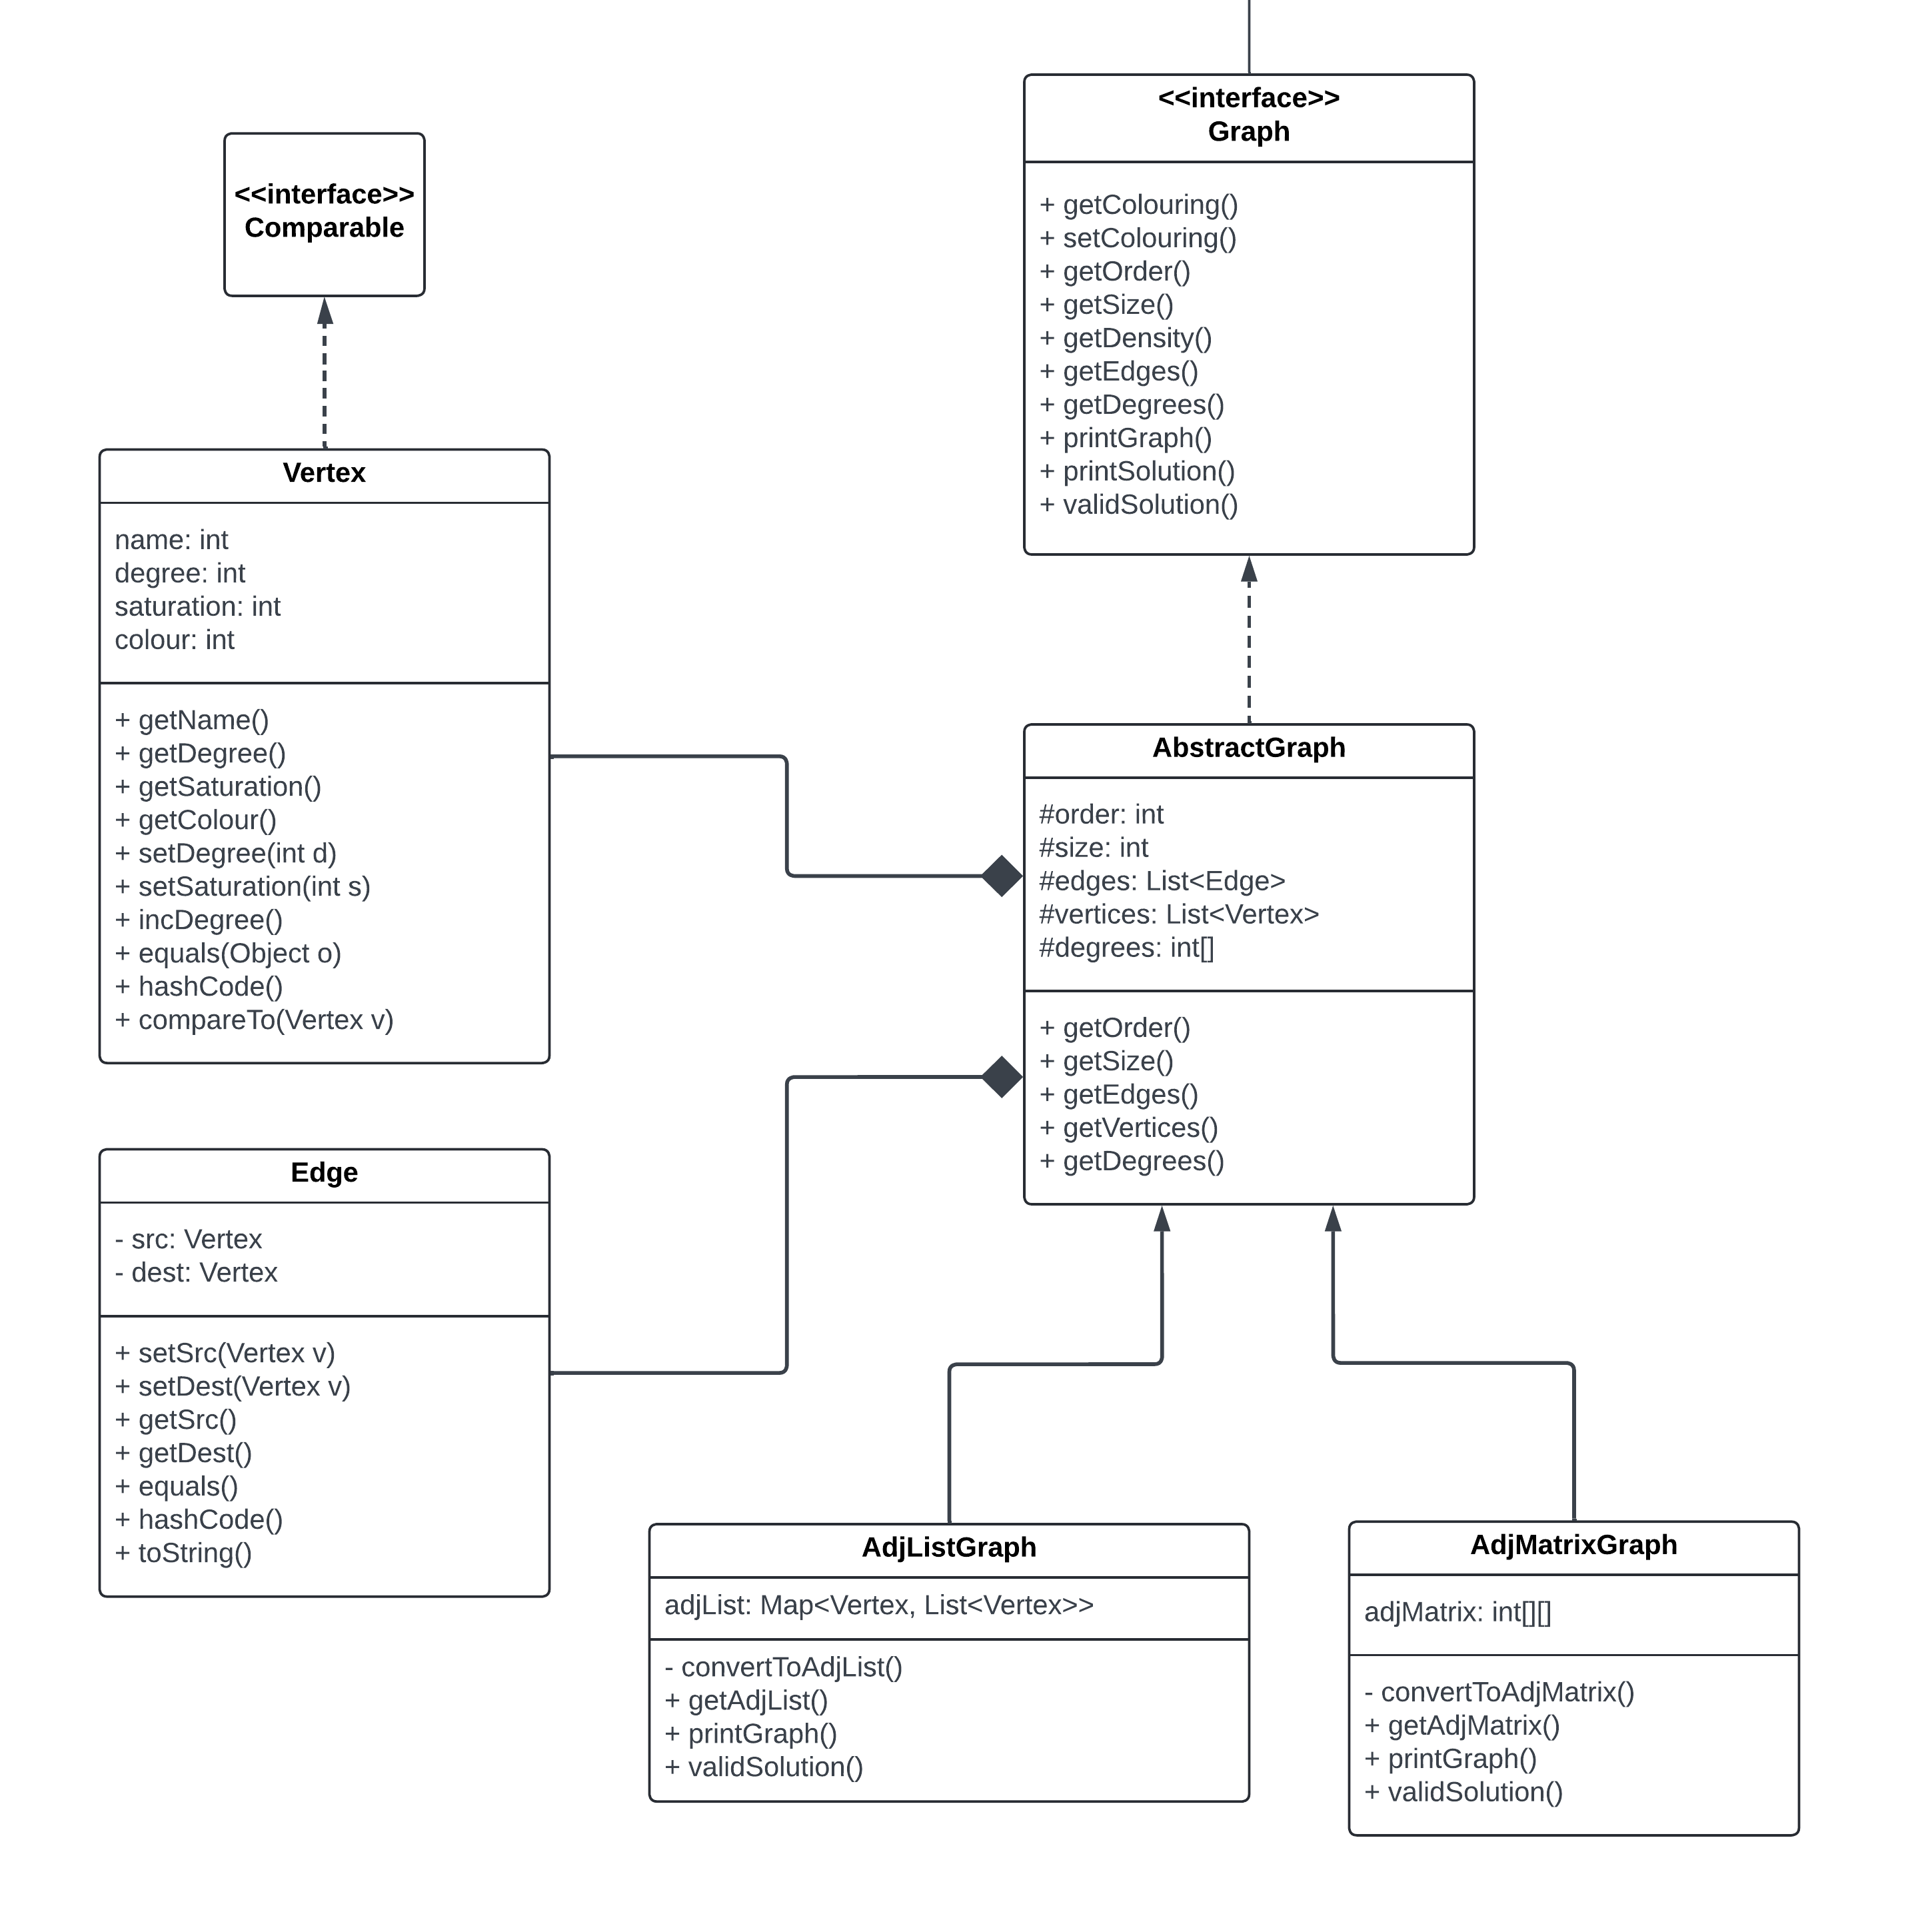
\includegraphics[width=0.9\linewidth]{Components/GraphHierarchy.png}
    \caption{UML class diagram showing the classes that make up the Graph Hierarchy}
    \label{fig:GraphHierarchy}
\end{figure}

The algorithms themselves (shown in Figure \ref{fig:GraphColouringHierarchy}) have been designed in a way to abstract anyone making use of them from their implementation. Each algorithm will have two methods that can be used to colour an input graph and to retrieve the number of checks or operations an algorithm must do to find a solution. A colouring will return a solution in the form of a Map that maps an integer colour to a set of vertices that make up the colour set. 
\\\\

\begin{figure}[H]
    \centering
    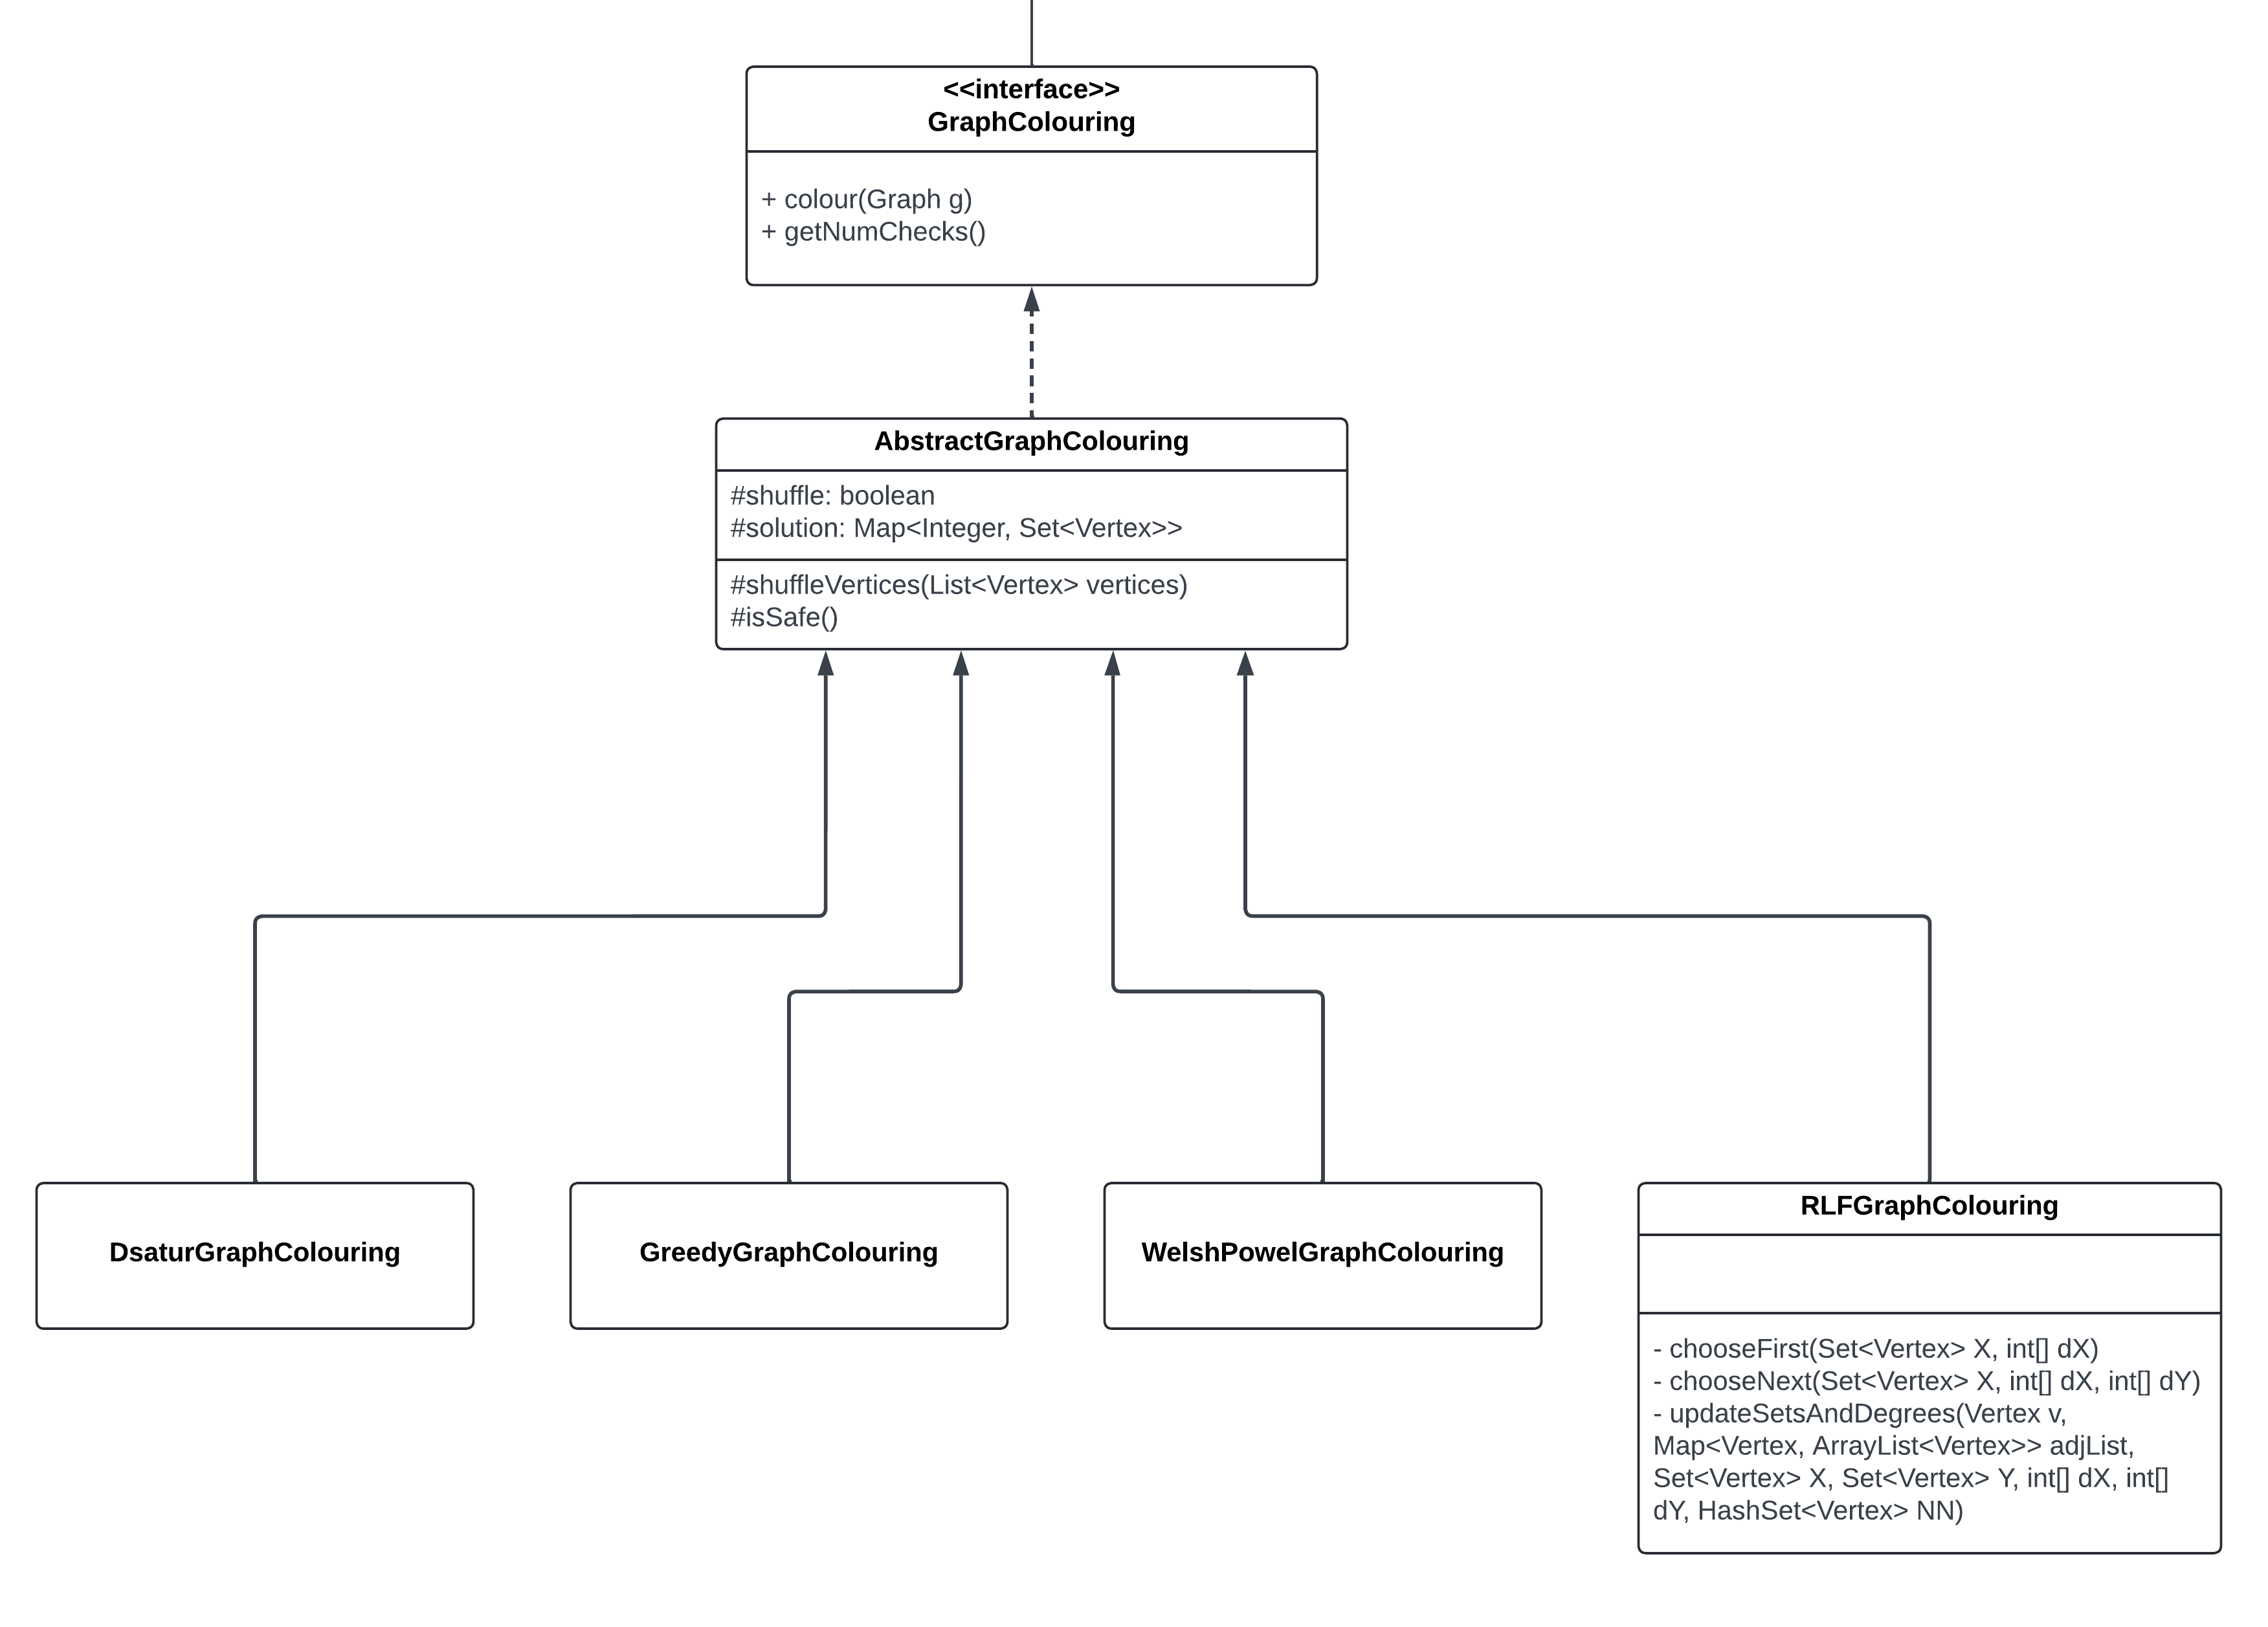
\includegraphics[width=0.9\linewidth]{Components/ColouringHierarchy.png}
    \caption{UML class diagram showing the classes that make up the Graph Colouring Algorithms Hierarchy}
    \label{fig:GraphColouringHierarchy}
\end{figure}

\begin{figure}[H]
    \centering
    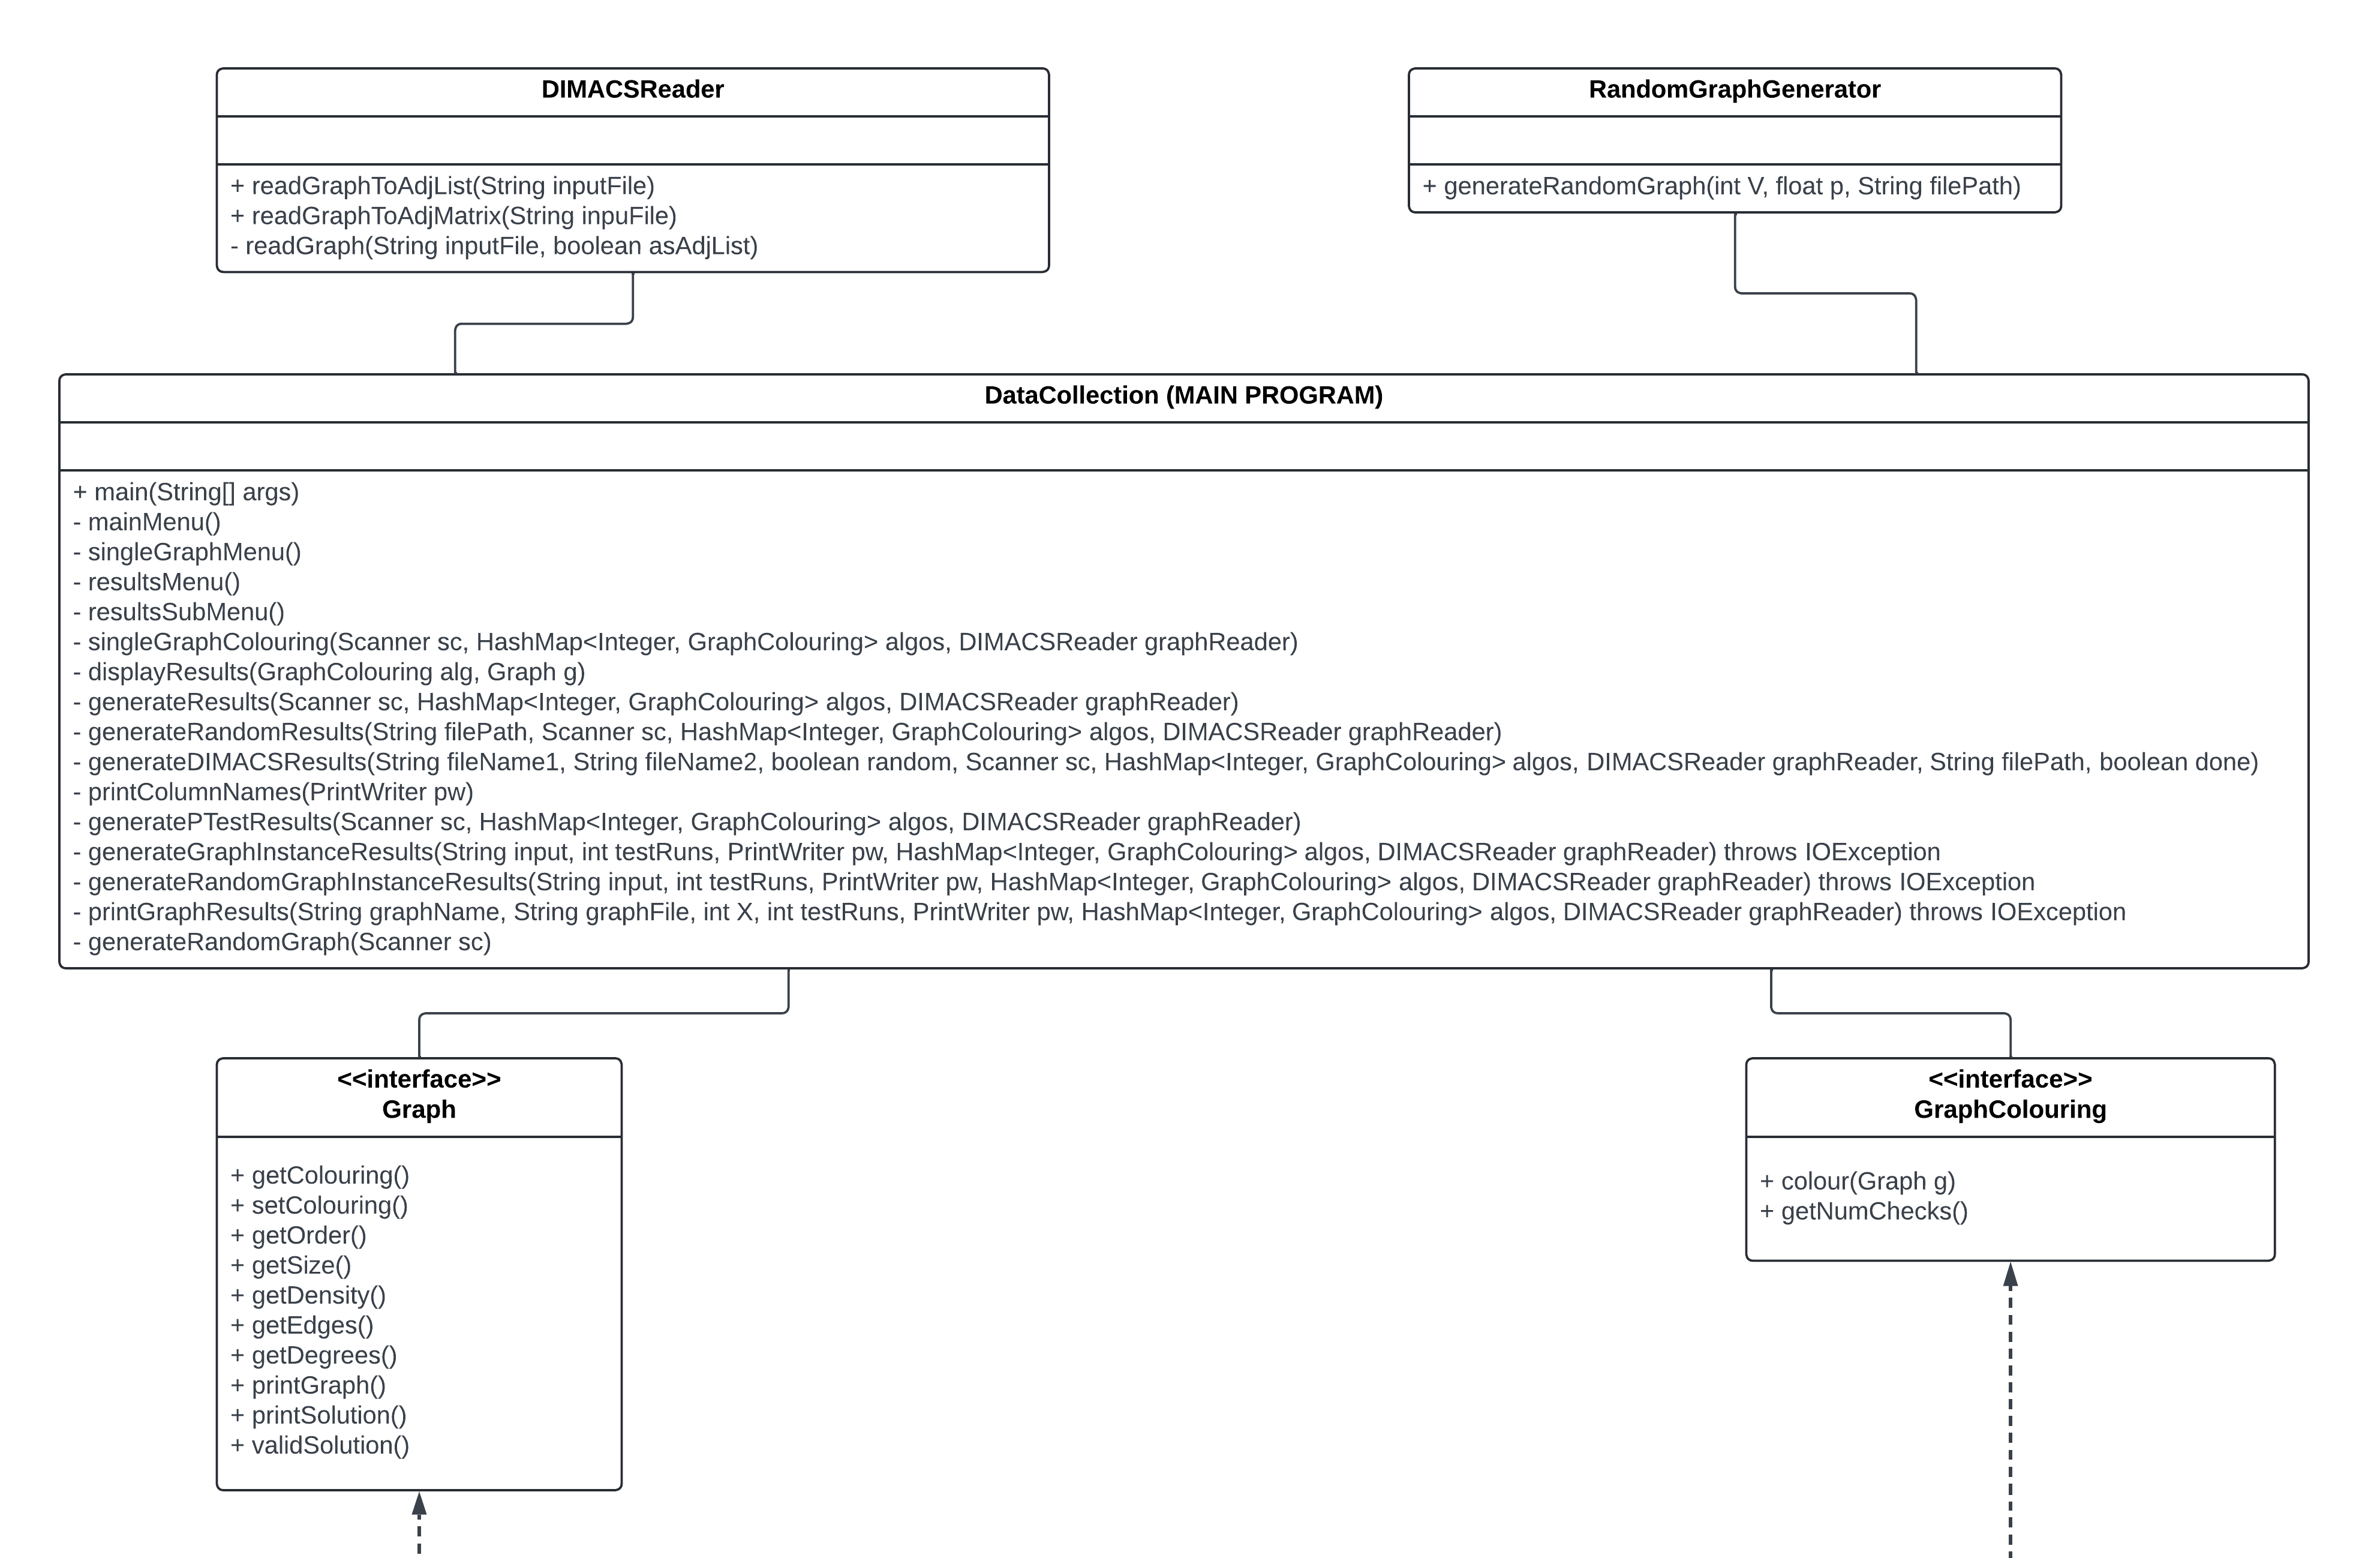
\includegraphics[width=0.9\linewidth]{Components/MainProgram.png}
    \caption{UML class diagram showing the classes that make up the Main Program}
    \label{fig:MainProgram}
\end{figure}

Finally, Figure \ref{fig:MainProgram} shows the design of the main program, along with the classes it uses to function. The main program is designed to provide a simple terminal UI that will satisfy the requirements set out in section 3.1. This includes a DIMACSReader class that allows for graphs to be read in from files. It also includes a RandomGraphGenerator class that has the ability to generate a random $G(n, p)$ graph and print it to an output file. 

\subsection{Implementation}
The following section provides some details into the implementation of the graph colouring software. The tasks for implementation were split into segments to mimic the idea of sprints in agile development. Each section typically follows chronologically from how they were implemented. As might be expected with agile development, however, each section was not necessarily developed independent from another. 

\subsubsection{Reading and Storing Graphs}
The first task was to find a way to read in DIMACS format graphs from an external file and then store them in a way that would be useful for running the algorithms on. The standardisation of the DIMACS format makes the reading of these files quite simple as a single method is required and it will never fail providing the file is in the correct format. The format is as follows:
\begin{verbatim}
    c lines beginning with c are a comment line 
    c describing the graph or any extra details
    c
    p edge Order Size
    e 1 2
    e 1 4
    .
    .
    .
\end{verbatim}
The lines  beginning with "c" are comment lines that provide the graph name and can include extra information about the graph such as density, chromatic number etc. For the purposes of reading in the graph the comment lines are generally ignored. The line starting "p" is where the reading in starts, this line provides the total number of vertices of the graph (Order) and the total number of edges (Size). This provides some useful information in order to set up the data-structures to store the information that is about to be read. The lines beginning with "e" are the graph itself. They are referred to as edge lines with the first number being one vertex and the second being another vertex. If two numbers share an edge line then they also share an edge. 
\\\\
In implementing the method to read the graph, considerations were made about disconnected vertices (i.e vertices that did not appear on an edge line), and handling bad input (such as incorrect file input, or incorrect file format). Important information that may be useful was also extracted from the reading process. This includes information about the degrees of each vertex, and the maximal degree vertex. 
\\\\
 In conjunction with building the method for reading in graphs, a storage hierarchy for the graphs themselves was being constructed. The hierarchy implemented closely follows the design set out in Figure \ref{fig:GraphHierarchy}. Each graph that is read in can be stored as either an Adjacency List graph or an Adjacency Matrix graph. A Graph is made up of Vertex and Edge objects. The reason for making a class of Vertex was to take advantage of the Comparable interface that Java provides. This allowed for ordering of Vertex objects within the constraints of some of the algorithms (i.e. in order of saturation for DSATUR or in order of degree for WELSH-POWELL). Similarly making a class of Edge allowed for checking if two edges are the same. This is necessary as graph colouring is done on directionless graphs so an edge $e\{1 \rightarrow 2\} \equiv e\{2 \rightarrow 1\}$. 
 
\subsubsection{Algorithms}
The algorithms themselves were the next part to be implemented. The following presents and explains the implementation, in pseudocode format, of the algorithms used in this project. Due to similarities between the GREEDY, SHUFFLED GREEDY and WELSH-POWELL1 algorithms, only the GREEDY pseudocode will be included. However, the slight variations between the three in implementation will be explained. 

\begin{figure}[H]
    \centering
        \begin{algorithm}[H]
        \DontPrintSemicolon
        \SetKwInOut{Input}{input}\SetKwInOut{Output}{output}
        
        \Input{A Graph G where $V$ is the set of Vertices and $A$ is the adjacency list}
        \Output{$S$ A Map of Coloured Vertex Sets}
        \BlankLine

        $S \leftarrow \emptyset$ \;
        \For{$v \in V$ \KwTo $|V|$}{
            $N \leftarrow A_{v}$ \;
            \For{$c \leftarrow 0$ \KwTo $|V|$}{
                \If{$!S_{c}$}{$S_{c} \leftarrow \emptyset$}
                Safe $\leftarrow True$ \;
                \For{$n \in N$ \KwTo $|N|$}{
                    \If{$n_{c} == c$}{
                        Safe $\leftarrow False$ \;
                        break \;
                    }
                }
                \If{Safe}{
                    $v_{c} \leftarrow c$ \;
                    $S_{c} \leftarrow S_{c} \cup \{v\}$
                }
            }
        }
        
        \caption{GREEDY}
        \end{algorithm}
    \caption{Pseudocode for the implementation of the GREEDY algorithm}
    \label{fig:GreedyImpPseudo}
\end{figure}

Figure \ref{fig:GreedyImpPseudo} shows the pseudocode of the implementation used for the GREEDY algorithm. Line 1 sets up $S$ (the solution to be returned) as an empty map, the map operates by mapping a colour, in this case an integer from $0 \rightarrow k$, to a set of vertices. The colour set created is denoted by $S_{c}$. Line 2 begins the loop iterating through every vertex of the graph. In the case of the GREEDY algorithm it will do this in order from $v_{1} \rightarrow v_{i}$ where $i$ is the order of the graph. Line 3 retrieves all the neighbours of the vertex $v$ from the adjacency list and assigns it to the variable $N$. On line 4 it starts looping through the colours in order to find a suitable colour, remembering that the GREEDY approach is to take the first feasible colour it can find. Lines 5-7 is a simple check that makes sure that if the colour has not been reached before then a new set will be constructed within the solution map. The main power of the GREEDY algorithm in providing correct solutions comes in lines 8-14. It loops through all the neighbours of $v$ and checks if the colour they have been assigned is the same as the current colour it is trying to assign to $v$. If it reaches any conflict it breaks out of the loop and moves on to the next colour. However, if it finds no conflicts it assigns $v$ with that colour and puts $v$ in the colour set $S_{c}$ as shown in lines 15-18. It then repeats the process for the the rest of the vertices until they have all been assigned a colour. 
\\\\
As mentioned previously the pseudocode for SHUFFLED GREEDY and WELSH-POWELL1 have not been included as they both build of the GREEDY method but simply change the ordering of the vertices. Therefore there is just one additional step required which is changing the order in which vertices are coloured. As mentioned in section 2 the SHUFFLED GREEDY method shuffles the vertices into a pseudo-random order using a random number generator to decide how to shuffle them. The WELSH-POWELL1 method sorts the vertices in order of their degree.

\begin{figure}[H]
    \centering
        \begin{algorithm}[H]
        \DontPrintSemicolon
        \SetKwInOut{Input}{input}\SetKwInOut{Output}{output}
        \SetKw{and}{and}
        
        \Input{A Graph G where $V$ is the Queue of Vertices (sorted by degree) and $A$ is the adjacency list}
        \Output{$S$ A Map of Coloured Vertex Sets}
        \BlankLine

        $S, X \leftarrow \emptyset$ \;
        $c \leftarrow 0$ \;
        \While{$|X| \neq |G|$}{
            $S_{c} \leftarrow \emptyset$ \;
            $v \leftarrow V_{first}$ \;
            $v_{c} \leftarrow c$ \;
            $S_{c} \leftarrow S_{c} \cup \{v\} $, $ X \leftarrow X \cup \{v\}$ \;
            \tcc{build set of non-neighbouring vertices of $v$}
            $N \leftarrow A_{v}, notN \leftarrow \emptyset$ \;
            \For{$u \in V$ \KwTo $|V|$}{
                \If{$u \notin N$}{
                    $notN \leftarrow N \cup \{u\}$
                }
            }
            \ForEach{$u \in notN$}{
                \tcc{same safety check as in GREEDY}
                \If{$u_{c} < 0$ \and Safe}{
                    $u_{c} \leftarrow c$ \;
                     $S_{c} \leftarrow S_{c} \cup \{u\} $, $ X \leftarrow X \cup \{u\}$ \;
                } 
            }
            $S \leftarrow S \cup S_{c}$ \;
            $c \leftarrow c + 1$
        }
       
        
        \caption{WELSH-POWELL2}
        \end{algorithm}
    \caption{Pseudocode for the implementation of the WELSH-POWELL2 algorithm}
    \label{fig:WP2ImpPseudo}
\end{figure}

Figure \ref{fig:WP2ImpPseudo} shows the implementation of the second variation of the WELSH-POWELL algorithm. The algorithm starts off by instantiating (initially empty) the map of $S$ (solution) and a set $X$ to keep track of which vertices have been coloured. On line 2 it starts by assigning the first colour to be constructed as 0, and line 3 begins the while loop within which each colour set will be constructed. Lines 4-7 show the process of selecting and colouring the first vertex of the colour set being constructed $S_{c}$. It selects the first vertex by taking the first vertex from $V$ (the queue of vertices). The first vertex being the one with the highest degree that has not yet been coloured. It then assigns the current colour to $v$ and adds it to the colour set $S_{c}$ and the set $X$ of coloured vertices. Lines 9-14 build a set containing all the vertices that are not a neighbour of $v$ meaning it may be eligible for the current colour set. Lines 15-21 go through the process of adding these candidate vertices to the colour set if: the candidate has not been coloured; and it is safe to do so (using the same safety check as in GREEDY). Finally, lines 22-23 show the constructed colour set being put in $S$ and increments to the next colour set to be constructed. The algorithm terminates when all the vertices have been assigned to a colour set. 

\begin{figure}[H]
    \centering
        \begin{algorithm}[H]
        \DontPrintSemicolon
        \SetKwInOut{Input}{input}\SetKwInOut{Output}{output}
        \SetKwFunction{uS}{updateSaturation}
        
        \Input{A Graph G where $V$ is the set of Vertices and $A$ is the adjacency list}
        \Output{$S$ A Map of Coloured Vertex Sets}
        \BlankLine

        $S \leftarrow \emptyset$,
        $Q \leftarrow V$ \;
        \While{$Q \neq \emptyset$}{
            $v \leftarrow Q_{first}$ \;
            $c \leftarrow 0$ \;
            \For{$c$ \KwTo $|V|$}{
                \If{$!S_{c}$}{$S_{c} \leftarrow \emptyset$}
                \If{Safe}{
                    $v_{c} \leftarrow c$,
                    $S_{c} \leftarrow S_{c} \cup \{v\} $
                }
            }
            \tcc{Remove $v$ from the graph and update the degrees and saturation of its neighbouring vertices in the induced subgraph}
            $N \leftarrow A_{v}$ \;
            \ForEach{$n \in N$}{
                \If{$n_{c} < 0$}{
                    $n_{d} \leftarrow n_{d} - 1$ \;
                    \uS{$n$} \;
                }
            }
        }
    
        \caption{DSATUR}
        \end{algorithm}
    \caption{Pseudocode for the implementation of the DSATUR algorithm}
    \label{fig:DSATURImpPseudo}
\end{figure}

Figure \ref{fig:DSATURImpPseudo} shows the implementation of the DSATUR algorithm. The algorithm starts off by using a Priority Queue denoted by $Q$ which works similarly to a heap data-structure. A heap is a type of tree data-structure where each parent node is either greater than (making a max heap) or less than (making a min heap) its child node. In this case $Q$ uses two constraints to order the vertices. The first and most important constraint is the saturation of the vertices. As established in section 2, saturation is the number of different colours that neighbour a vertex. The second constraint is the degree of the vertex. In short, vertices with the highest saturation are placed at the front of $Q$. If multiple vertices have the same saturation then the vertex with the highest degree comes first. If vertices have the same saturation and the same degree then the choice is arbitrary, in this case the vertex with the lowest label is chosen. This method of ordering is where the main power of DSATUR comes from. It then assigns the minimum colour it can to each vertex $v$. Therefore, on line 3, the algorithm chooses the first vertex from $Q$ given the constraints just established, and removes it from $Q$. Lines 4-12 are almost identical to that of the GREEDY algorithm simply choosing the minimal safe colour to assign to the vertex $v$. Lines 14-20 are bookkeeping to ensure the saturation and degrees of each neighbouring vertex of $v$ is updated for the next iteration. The process then repeats for the next vertex until all vertices are coloured, in this case when $Q$ is empty. 

\begin{figure}[H]
    \centering
        \begin{algorithm}[H]
        \DontPrintSemicolon
        \SetKwInOut{Input}{input}\SetKwInOut{Output}{output}
        \SetKwFunction{uDAS}{updateSetsAndDegrees}
        
        \Input{A Graph G where $V$ is the set of Vertices and $A$ is the adjacency list}
        \Output{$S$ A Map of Coloured Vertex Sets}
        \BlankLine

        $S \leftarrow \emptyset$ \;
        $X \leftarrow V$, $Y \leftarrow \emptyset$ \;
        $c \leftarrow 0$ \;
        \While{$X \neq \emptyset$}{
            $S_{c} \leftarrow \emptyset$ \;
            $v \leftarrow X_{first}$ \;
            $v_{c} \leftarrow c$,
            $S_{c} \leftarrow S_{c} \cup \{v\}$ \;
            \uDAS{$v$, $X$, $Y$} \;
            \While{$X \neq \emptyset$}{
                $u \leftarrow X_{next}$ \;
                $u_{c} \leftarrow c$, 
                $S_{c} \leftarrow S_{c} \cup \{u\}$ \;
                \uDAS{$u$, $X$, $Y$}
            }
            $S \leftarrow S \cup S_{c}$ \;
            $X \leftarrow Y$ \;
            $Y \leftarrow \emptyset$ \;
            $c \leftarrow c + 1$
        }
    
        \caption{RLF}
        \end{algorithm}
    \caption{Pseudocode for the implementation of the RLF algorithm}
    \label{fig:RLFImpPseudo}
\end{figure}

Finally, the implementation of RLF is shown in Figure \ref{fig:RLFImpPseudo}. The algorithm sets out by introducing two distinct sets that will be used throughout the algorithm to keep track of the vertices. The set $X$ holds the vertices that are candidates (initially all vertices) to be included within $S_{c}$, the colour set being constructed. Whereas, $Y$ holds the vertices that are not eligible to be included within $S_{c}$ (initially empty). On lines 6-7 the first vertex $v$ is selected from the candidate vertices in $X$ based on the vertex with maximal degree (any ties make selection arbitrary, as in DSATUR the vertex is chosen based on smallest label). On line 8 there is a call to a method that updates $X$ and $Y$ based on the vertex $v$ that is being coloured. All the neighbours of $v$ are placed in $Y$ as they can no longer be considered for $S_{c}$. The heuristics for the next vertex $u$ to be coloured (as established in section 2) are determined by the vertex with the most neighbours in $Y$. This process, shown on lines 9-13, is repeated until there are no candidates left in $X$. The colour set $S_{c}$ is then stored in $S$. All the vertices in $Y$ are moved over to $X$, and $Y$ is emptied. The process then starts over again constructing the next colour set until all the vertices of the graph have been coloured.  

\subsubsection{Random Graph Generator}

The next thing to be implemented was a method to generate random $G(n,p)$ graphs to test the algorithms on. This was made simple using  Java's inbuilt Random class. The method requires an input value of $n$ (being the total number of nodes of the graph being generated), and also a value for $p$ (being the probability that two vertices will share an edge). After that the method simply loops through all the possible edges of the graph and uses the random generator to determine if an edge will be created or not. An edge is created if the value that is generated by Random is smaller than $p$. The resulting graph is then printed to an output file in DIMACS format, along with some useful information, in the form:
\begin{verbatim}
    c File: {graph_name}
    c 
    c This is a randomly generated graph G(n, p) where: 
    c n (num vertices): {n_input}
    c p (edge probability): {p_input}
    c 
    c Graph Properties: 
    c Order: {n_input}
    c Size: ...
    c Density: ...
    c Maximum Degree: ...
    c Minimum Degree: ...
    c Average Degree: ...
    c 
    p edge Order Size
    e 1 5
    e 1 9
    .
    .
    .
\end{verbatim}

This allows for multiple $G(n,p)$ graphs to be generated and means that a user can utilise and reflect back on the useful information provided regarding the graphs topology. 

\subsubsection{Main Program}
The final stage of implementation was to create a simple terminal based UI in order to generate the results required to achieve the project aims. Figure \ref{fig:MainMenu} shows the main menu of the terminal program. This was implemented to satisfy the functional and non-functional requirements set out in section 3.1 Table \ref{tab:FuncReqs} and Table \ref{tab:NonFuncReqs} respectively. Option 1 allows users to test the algorithms on a single test instance, thus satisfying FR1. Option 2 allows users to generate results on various DIMACS test instances, satisfying FR9. Option 3 allows for the generation of results testing the algorithms on $G(n, p)$ graphs, satisfying FR10. Option 4 allows for the generation of a new $G(n, p)$ graph, satisfying FR11. Finally, option 5 allows the user to quit the program, satisfying FR13 and NFR6. 
\begin{figure}[H]
    \centering
    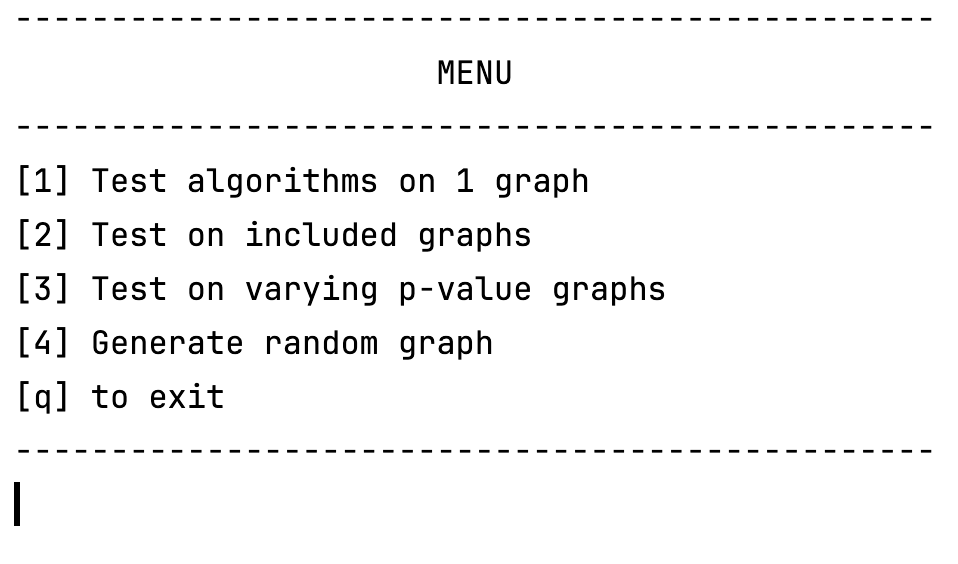
\includegraphics[width=0.5\linewidth]{Components/MainMenu.png}
    \caption{Main Menu of the terminal program}
    \label{fig:MainMenu}
\end{figure}

After selecting option 1 on Figure \ref{fig:MainMenu} the program prompts you to input a graph file path and directs you to the algorithm selection menu as shown in Figure \ref{fig:AlgSelect}. The user may then select which algorithm (or input 6 to select all) to use and the program will print the results to the terminal. If the user provides any incorrect input, they will be directed to start the process again. This satisfies FR2-FR8 and NFR2. 

\begin{figure}[H]
    \centering
    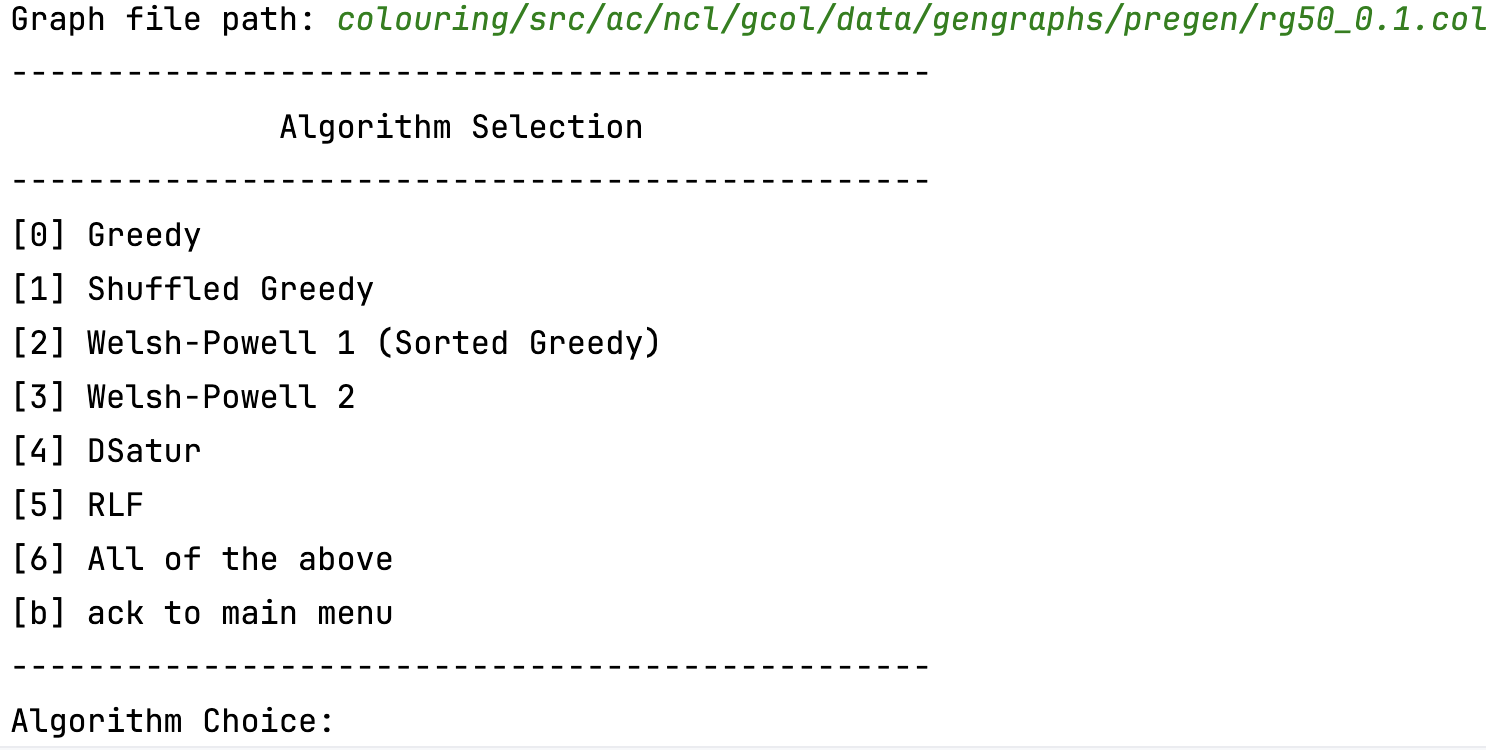
\includegraphics[width=0.5\linewidth]{Components/AlgorithmSelection.png}
    \caption{Algorithm selection menu for colouring a single graph}
    \label{fig:AlgSelect}
\end{figure}

After selecting option 2 from Figure \ref{fig:MainMenu} the user will be directed to choose the type of graph instance they wish to generate results for, as shown in Figure \ref{fig:GtypeSelect}. The program will then run the algorithms on the desired test instances and output the results to a CSV file. The results will include the number of colours $k$ each algorithm uses, the number of operations each algorithm performs, and the time (in nanoseconds) it takes for an algorithm to find the solution. If the user provides any incorrect input, they will be directed to start the process again. This satisfies NFR3. 
\begin{figure}[H]
    \centering
    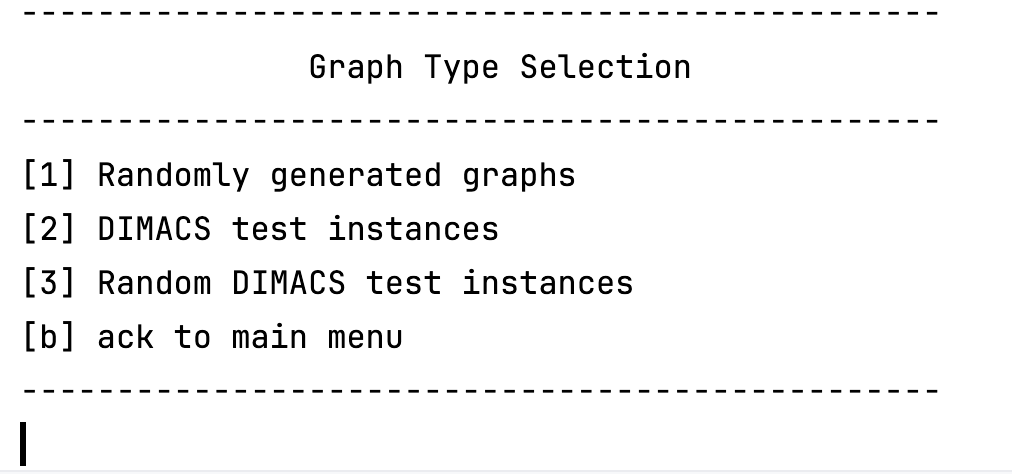
\includegraphics[width=0.5\linewidth]{Components/GraphTestSelection.png}
    \caption{Graph type selection menu for testing algorithms and generating results}
    \label{fig:GtypeSelect}
\end{figure}
After selecting option 3 from Figure \ref{fig:MainMenu} the user will be directed to answer questions regarding the types of $G(n, p)$ graph they would like to test on. The first question the user will be asked is the number of variations of $G(n, p)$ to generate per $p$-value. Then, users will be asked to input the desired $p$-values to test on in a comma separated list. Finally, users will be asked to input a value for $n$ (the number of nodes). The program will then generate the desired results and output these to a CSV file. The results will be in the same format as those generated from option 2. If the user provides any incorrect input, they will be directed to start the process again. This satisfies NFR4.
\begin{figure}[H]
    \centering
    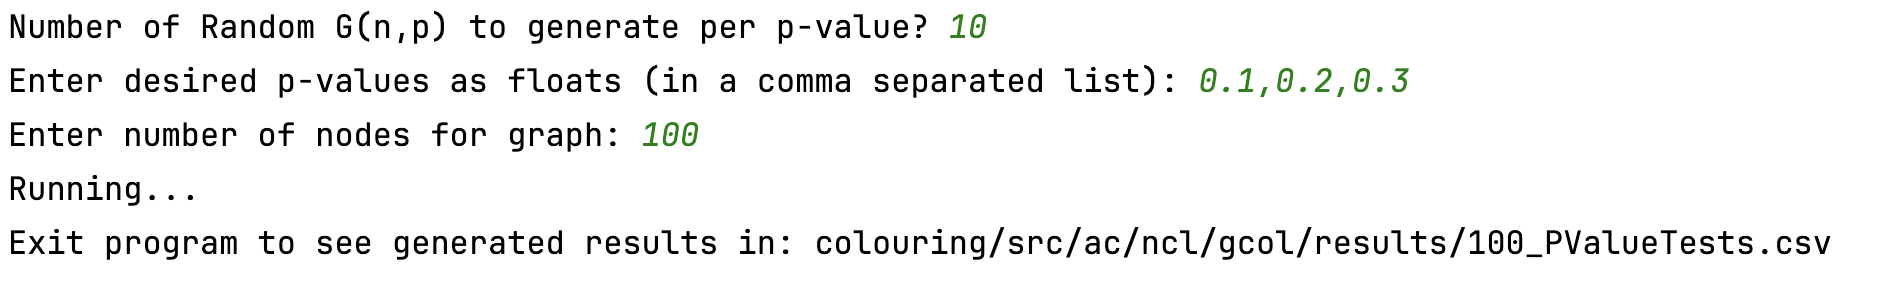
\includegraphics[width=0.7\linewidth]{Components/RunningTests.png}
    \caption{Running algorithms and generating results for $G(n, p)$ graphs}
    \label{fig:enter-label}
\end{figure}
After selecting option 4 from Figure \ref{fig:MainMenu} the user is prompted to input a value for $n$ and a value for $p$. The graph is then generated and outputted to a file in DIMACS format. This satisfies NFR5.

\subsection{Testing}
Due to the time constraints of this project, formal unit testing was not feasible. Instead, several checks were performed whilst the program was being implemented. Firstly, whilst building the graph reader it was ensured that all information stored within the graph objects matched the information of the input file. For example, it was ensured that the density, maximal degree, and average degree of the vertices were the same in both. Secondly, whilst building the graph storage, small graph instances were visually inspected (by printing to the terminal) to ensure they matched the input file. For the algorithms themselves several testing methods were adopted. In some cases (specifically in small test instances) solutions were generated by hand to ensure that the solution generated by the program was accurate. In other cases, the result was checked against known results for the particular algorithm to ensure accuracy. A method was created to ensure that all solutions generated were correct solutions (i.e. there were no colouring conflicts). With regard to the random graph generator, it was ensured that the $p$-value chosen and the density of the graph were similar (as these are linked). Finally, with regards to the main program, user testing was performed iteratively during the development process to ensure that features worked as expected and were in accordance with the requirements.
\\\\
In terms of testing the algorithms performance against the metrics established in the aims of this project, the decision was made to test $G(n, p)$ graphs with varying $n$ and $p$-values and test DIMACS instances with known chromatic numbers. As $p$-values and density are linked, increasing $p$ will increase the density of the graph. Therefore, decision to test $p$-values 0.1, 0.2, 0.3, 0.4, 0.5, 0.6, 0.7, 0.8, and 0.9 was made because it will allow the author to measure the algorithms performance on a variety of graphs from those that are sparse to those that are extremely dense. This will allow the author to see the effectiveness and efficiency of the algorithm as the graph becomes denser. Likewise, altering $n$ values will have a similar effect. Therefore, the decision was made to test $n$ values of 50, 100, 150, 300, 500, 750, 1000, and 1500 as this will provide sufficient difference in number of nodes to see change in algorithm effectiveness and efficiency, whilst being small enough to be manageable within the time constraints. 20 test runs were performed per value of $p$ to provide averages for the number of colours used, number of operations performed, and time taken.
\\\\
Testing only DIMACS instances with known chromatic numbers was also performed, as this provides a metric to determine the effectiveness of the algorithms by comparing the difference between the number of colours used and the chromatic number of the graph. A list of the graphs can be seen in Table \ref{tab:DIMACSResults} (section 4.3). These graphs were taken from the second DIMACS implementation challenge \cite{DIMACSChallenge2}. Leighton's random graphs with known chromatic numbers (shown in Table \ref{tab:LeightonGraphResults}, section 4.4), were also tested to provide a similar metric to determine the effectiveness of the algorithms. The format of this table is based on the table presented by Leighton in his seminal formulation of the RLF algorithm \cite{Leighton1979AGC}. Similar to tests on $G(n, p)$ graphs, 20 test runs were performed per value of $p$ to provide averages for the number of colours used.
